\documentclass{article}
\usepackage{graphicx}
\usepackage[sorting=none]{biblatex}
\addbibresource{library.bib}
% \usepackage[utf8]{inputenc}
\usepackage[russian]{babel}
\usepackage{hyperref}
\usepackage[letterpaper,top=2cm,bottom=2cm,left=3cm,right=3cm,marginparwidth=1.75cm]{geometry}
\title{Домашнее задание}
\date{}
\begin{document}
\maketitle

Время жизни куперовсих пар в ферромагнетике может быть увеличеною Если в SF структуре имеется пространственная неоднородность намагниченности, то могут возникать триплетные корреляции с ненулевым спином \cite{bergeret2001long, kadigrobov2001quantum}. Тогда обменное взаимодействие уже не стремится разорвать пары, и они глубоко проникатют в ферромагнетик, распространяясь на сотни нанометров \cite{keizer2006spin}. 
\begin{figure}[h]
    \centering
    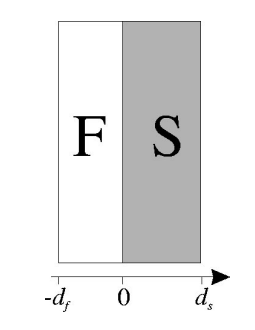
\includegraphics{FS.png}
    \caption{FS структура. Ферромагнетик занимает область $-d_f<x<0$, а сверхпроводник $0<x<d_s$}
    \label{FS}
\end{figure}

Для описания гибридных структур в "грязном" пределе используются уравнения Узаделя:
\[\Phi = \Delta + \frac{D}{2\omega}\frac{\partial}{\partial x}G^2\frac{\partial \Phi}{\partial x}\]
\[\Delta \ln \frac{T}{T_c} = \pi T \sum\limits_\omega \frac{\Delta - \Phi G}{\omega}\]
\[\xi_2 G_2^2 \frac{\partial \Phi_2}{\partial x} = \gamma\xi_1 G_1^2 \frac{\partial \Phi_1}{\partial x}\]
\[\xi_2 \gamma_B G_2 \frac{\partial \Phi_2}{\partial x} = G_1(\Phi_1 - \Phi_2)\]
где $G$ - нормальная компонента функции Грина, $F$ - аномальная компонента функции Грина, а $\Phi$ - параметр, которые связаны соотношениями:
\[G = \frac{\omega}{\sqrt{\omega^2 + \Phi\Phi^*}}, \; \; F = \frac{\Phi}{\sqrt{\omega^2 + \Phi\Phi^*}} = \frac{G\Phi}{\omega}\]
$\gamma$ и $\gamma_B$ - параметры, характеризующие границу 
\[\gamma_B = \frac{R_B}{\rho_1 \xi_1} \; \; \gamma = \frac{\rho_2\xi_2}{\rho_1\xi_1}\]
$\xi_1, \; \xi_2$ и $\rho_1, \; \rho_2$ длины когерентности и сопротивления участков 1 и 2, соответственно. $\xi_{1,2} = \sqrt{D_{1,2}/2\pi T_cs}$, $D_{1,2}$ - коэффициент диффузии.
\newline $\omega = \pi T (2n+1)$ частота Мацубары. В ферромагнетике $\omega_F = \omega + iH$

Рассмотрим структуру на рис.1. Можно перейти к линейному приближению и положить в уравнениях $\Phi=1$, тогда после преобразований получим систему:
\begin{equation}
    \xi_s^2\pi T_{cs}\frac{d^2 F_s}{d x^2} - |\omega_n|F_s + \Delta = 0, \; \; 0<x<d_s
\end{equation}
\begin{equation}
    \xi_f^2\pi T_{cs}\frac{d^2 F_f}{d x^2} - (|\omega_n| + iE_{ex}sgn\: \omega_n)F_f = 0, \; \; -d_f<x<0
\end{equation}
\begin{equation}
    \Delta \ln \frac{T_{cs}}{T} = \pi T \sum\limits_{\omega_n}\left( \frac{\Delta}{|\omega_n|} - F_s\right)
\end{equation}

\printbibliography
\end{document}
